% Requires graphicx. Paths are relative to this snippet.
\begin{figure*}[t]
\centering
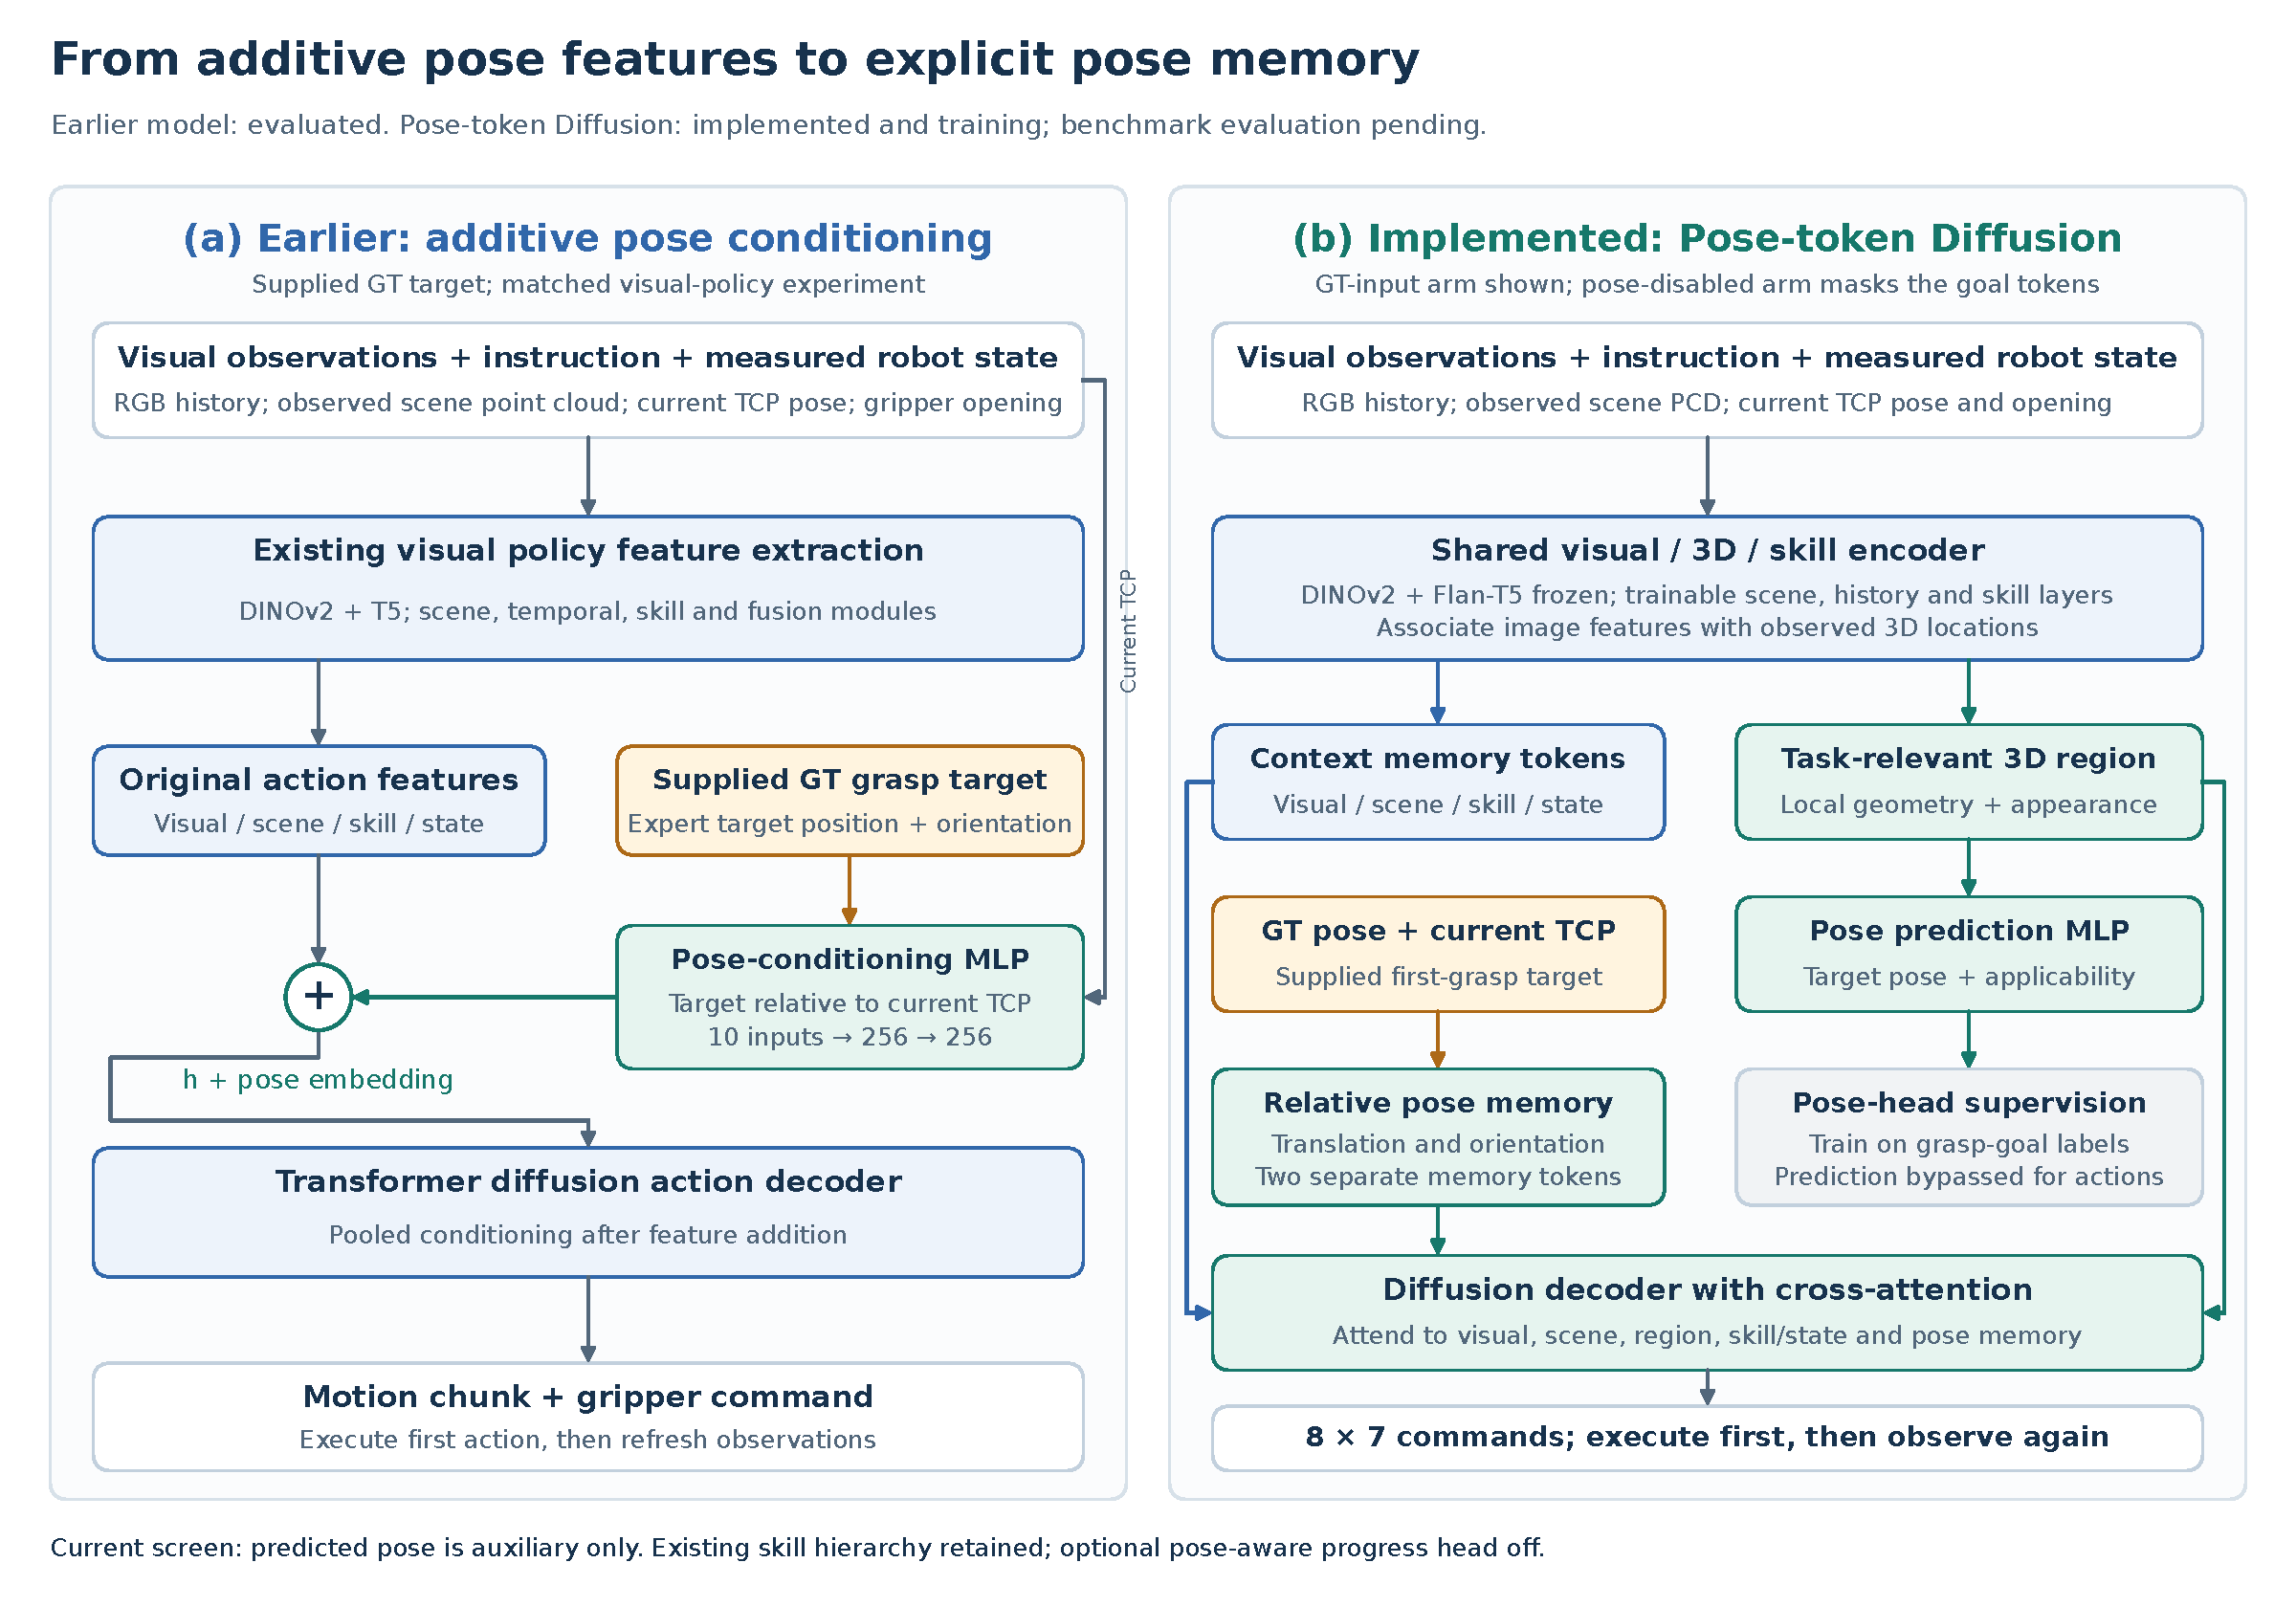
\includegraphics[width=\textwidth]{old_vs_implemented_pose_token_diffusion.pdf}
\caption{Earlier additive GT-pose conditioning and the implemented Pose-token
Diffusion policy. Both retain visual and measured robot-state inputs. The new
policy associates RGB and scene geometry, grounds a task-relevant region, and
encodes the selected goal as distinct relative translation and orientation
tokens for a cross-attention diffusion decoder. The current GT-input arm supplies
an expert first-grasp target. The pose-disabled arm masks goal tokens. Both arms
train an auxiliary pose head whose predictions do not condition actions in this
screen. Predicted-goal conditioning is supported for subsequent study. The
existing skill hierarchy remains active; the optional pose-aware progress head
is disabled. The new full-training comparison has no benchmark result yet.}
\label{fig:implemented-pose-token-comparison}
\end{figure*}
